\graphicspath{{./images/}}      
\def\CHAPTERONE{./chapters/Chapter-1} 

\chapter{Grundlagen}
\label{chap:software}
%	\input{\CHAPTERONE /motivation}
\glsresetall
\section{\unreal}
\label{sec:unrealengine}
Die von Epic Games\footnote{\url{https://www.epicgames.com}} entwickelte \unreal\footnote{\url{https://www.unrealengine.com}} ist eine \gls{gameengine} zur Entwicklung von Videospielen und zur Erstellung von filmischen Erfahrungen \cite{featUnreal}. Mittlerweile befindet sich die \unreal in ihrer vierten Generation und enthält neben der \acrshort{engine} selbst auch eine Vielzahl an Werkzeugen, die den Workflow der Nutzer vereinfachen und effizienter gestalten. Erhältlich ist die \acrshort{engine} für die Betriebssysteme Windows, MacOS und Linux. \par

Im Kern bietet die \unreal eine Möglichkeit zur Echtzeitmanipulation und Erstellung von Anwendungen wie Videospielen. Dazu gehören zum Beispiel fotorealistisches Rendering, \gls{vr}-Unterstützung und Entwicklung, ein Partikel- und VFX-System, sowie ein KI-System. Weitere Tools umfassen unter anderem einen Animator und einen Sequencer, der zur Erstellung und Editierung von filmischen Sequenzen genutzt werden kann. \par 

Seit Februar 2015 ist der C++ Quellcode der \unreal offen verfügbar und die \acrshort{engine} kostenlos nutzbar, solange kein Gewinn in einer bestimmten Höhe erzielt wird \cite{freeUnreal}. Im Zuge dessen kann jeder Nutzer an der Entwicklung der \acrshort{engine} teilhaben und/oder sie für seine persönlichen Zwecke individualisieren. Zusätzlich können auf dem \textit{Marketplace} zusätzliche Inhalte und Plugins von Drittanbietern erworben und in die \acrshort{engine} integriert werden, wodurch die \unreal ein hohes Maß an Flexibilität und Individualisierung bietet. \par 

Für diese Arbeit interessant ist das fotorealistische Rendering in Echtzeit: die \unreal bietet damit eine Möglichkeit in einer \acrfull{vr} 3D-Szenarien zu erstellen, von denen Bilder als Trainingsdaten für ein \gls{mln} geschossen werden können. Natürlich setzt das voraus, dass die Objekte und Umgebung in der zu rendernden Szene auch realistische Modelle besitzen.     

\subsection{Küchen Umgebung}
\label{subsec:kitchenenvironment}
Um in einer Game Engine ein zu spielendes \textit{Level} (oder \textit{Map}) mit Objekten, mit denen der Spieler interagieren kann, zu füllen, braucht man sogenannte \textit{Assets}. Dies sind 3D-Modelle, die in einem 3D-Modellierungsprogramm erstellt oder mit einem 3D-Scanner eingescannt wurden. Das Rendern der Modelle passiert während der sogenannten Simulation. Wenn diese gestartet wird, kann das Level im Sinne seiner Programmierung \glqq gespielt\grqq \ werden. In diesem Fall ist es jedoch nicht vorgesehen, das ein Spieler in der Welt bewegt oder mit ihr interagiert. Stattdessen wird nur eine Kamera eingesetzt, die von dem durch die Modelle gezeigten Szenario Bilder erzeugt.  \par
Das \gls{iai} besitzt \textit{Assets} für eine realistische Küchenumgebung. Diese ist eine Nachbildung einer echten zu Forschungszwecken verwendeten Küche im Institut und wird im Rahmen des Projekts \robcog\footnote{\url{http://www.robcog.org/}} ständig verbessert und erweitert. Das Ziel von \robcog ist es Roboter über \textit{Serious Games} mit Commonsense und physikalischem Wissen auszustatten. Da bei dem Erstellen und Abnehmen eines Bildes aus der \acrshort{engine} kein Bedarf besteht Schubladen zu öffnen, Objekte anzuheben oder die Herdplatten anzustellen, wird eine Version der Küche benutzt, die auf solche Funktionen verzichtet.\footnote{\url{https://github.com/robcog-iai/RobCoG/tree/dev-env}} \par
Die Objekte des täglichen Bedarfs, die im Rahmen dieser Arbeit erkannt werden sollen, sind auch Teil der Küchenumgebung. Es handelt sich bei ihnen um eingescannte echte Objekte, sodass sie einen hohen Detail- und Realitätsgrad besitzen und sich auch in der echten Küche finden. Für eine Liste aller benutzten Objekte siehe Tabelle \ref{tab:objects} auf Seite \pageref{tab:objects}.
 
\subsection{URoboVision}
\label{subsec:urobovision}
Damit die Bilder aus der \unreal von der Perzeptionspipline in \robosherlock verarbeitet werden können, wird ein \unreal Plugin verwendet. URoboVision\footnote{\url{https://github.com/robcog-iai/URoboVision}} bietet eine simulierte RGBD-Kamera in Form eines in die Map einfügbaren \textit{ARGBDCameraActor}, der die benötigten Informationen aus der \unreal zieht und dann über eine TCP-Verbindung an \robosherlock schickt.  Dazu werden drei Bilder, ein Farbbild, ein Tiefenbild, und eine Objektmaske von der Szene erzeugt. Letzteres ist ein Bild, in dem jedes Objekt in einer anderen Farbe eingefärbt ist. Zusätzlich wird noch eine Map übermittelt, in der jeder Farbe ein eindeutiger Objektname, nämlich der Asset-Name des Modells, zugeordnet ist. Daraus kann später die Groundtruth für Objekthypothesen  ermittelt werden. Über verschiedene Parameter kann die Kamera individuellem Vorgehen angepasst werden. \par 

\subsection{RSpawnBox}
\label{sec:rspawnbox}

Im Rahmen des Bachelor Projekts UnrealRobots im WiSe16/17\&SoSe17 der Universität Bremen wurde von mir im VisionScanning-Subprojekt\footnote{\url{https://gitlab.informatik.uni-bremen.de/dieckmdo/P12-VisionScanning-UR16} GitLab Account der Universität Bremen notwendig} die RSpawnBox Klasse für die \unreal implementiert. Diese bietet die Möglichkeit ausgewählte Objekte innerhalb eines Bereichs (einer \textit{Bounding Box}) an zufälligen Plätzen erscheinen zu lassen. Zusätzlich rotierte eine Kamera in anpassbarem Abstand und Winkel um die erschienenen Objekte. Im Rahmen dieser Arbeit wurde letzterer Teil der Klasse in modifizierter Form verwendet, um Bilder aus verschiedenen Ansichten der Szene mit der URoboVision Kamera aufzunehmen. Mehr dazu in Kapitel \ref{sec:takingpics}.         

\section{ROS}
\label{sec:ros}
Das \gls{ros}\footnote{\url{http://www.ros.org}} ist ein quelloffenes, modular designtes \gls{framework} für die Entwicklung von Robotersoftware. \gls{ros} bietet dafür eine Kommunikationsebene über dem Betriebssystem der einzelnen Computer innerhalb eines Robotersystems und eine Menge hilfreicher Werkzeuge an \cite{ros}.\par 

Zu Grunde liegt dem eine Peer-to-Peer Topologie, sodass theoretisch jeder Prozess oder Computer mit jedem anderen kommunizieren kann. Dank eines Programmiersprachen-neutralen Designs ist dies auch über verschiedene Sprachen hinweg kein Problem und ermöglicht so die Berücksichtigung der Bevorzugung bestimmter Sprachen für bestimmte zu implementierende Probleme, als auch Präferenzen des Entwicklers.\par

Die Kommunikation läuft über sogenannte \textit{Nodes}. Ein Node ist ein Prozess der eine bestimmte Aufgabe bearbeitet. Der Datenaustausch findet nun über \textit{Topics} oder \textit{Services} statt. Beide haben eindeutig identifizierbare Namen und Nodes können sich an ihnen als \textit{Publisher} anmelden oder als \textit{Subscriber} auf sie horchen. Nodes, die als Publisher tätig sind, veröffentlichen nun auf der gegebenem Topic oder Service Daten, während Subscriber die Daten von den entsprechenden Topics oder Services erhalten. Der Unterschied besteht darin, dass Services einmalig sind, während es mehrere Nodes geben kann, die Daten auf einer bestimmten Topic veröffentlichen. Der Austausch von Daten passiert dann in Form von \textit{Messages}. Dies sind feste Datenstrukturen, zum Beispiel die primitiven Datentypen integer und boolean, aber auch Arrays und Messages selbst. \par

\gls{ros} kommt mit einer Reihe von Werkzeugen, die in jeweils eigenen Modulen implementiert sind, um so erhöhte Stabilität und verringerte Komplexität zu erreichen. Das Kernmodul, der \textit{ROS-master}, enthält somit nur die Kernfunktionalität. Die zusätzlichen Werkzeuge ermöglichen unter anderem das Debuggen einzelner Nodes, die Visualisierung des Datenaustausches oder einzelner Topics, das Starten ganzer Node-Verbünde und die mehrfach Instanziierung von solchen, sowie das Erstellen von \textit{ROS-Packages}. Letzteres erlaubt das Aufteilen einzelner Funktionalitäten in Pakete und so das einfache Zusammenarbeiten mehrerer Entwickler. Jedes Paket kann jeweils seine eigenen Drittbibliothek-und Paketabhängigkeiten haben, sowie auch auch beliebig tief geschachtelt werden. Ein Paket kann also aus weiteren Paketen bestehen, wie zum Beispiel das im Rahmen dieser Arbeit verwendete \robosherlock. Zum Zeitpunkt dieser Arbeit existieren über 3000 öffentliche ROS-Packages.   

\section{\robosherlock}
\label{sec:robosherlock}
\robosherlock\footnote{\url{http://robosherlock.org/}} ist ein quelloffenes \gls{framework} zur Implementierung von Roboter Perzeptionssystemen. Dabei bietet \robosherlock auch die Möglichkeit, Wissen zu akquirieren, indem Objekte auf Eigenschaften analysiert werden, und darüber zu Schlussfolgern, als auch Fragen zu der wahrgenommenen Szene zu beantworten. Dabei bekommt der Roboter die Aufgabe nach Objekten einer bestimmten Beschreibung Ausschau zu halten und kann über diese dann zusätzliche Informationen erfahren \cite{robosherlock}. \par
\robosherlock basiert auf der \textit{unstructred information management architecture (UIMA)}\footnote{\url{https://uima.apache.org/}}. Dabei werden Dokumente als unstrukturiert angesehen, weil ihnen eine explizite Bedeutung fehlt, die Maschinen bräuchten, um die Informationen aus ihnen zu Interpretieren. Beispiele für solche Dokumente sind natürlichsprachliche Texte, Bilder und Videos. Ziel von UIMA ist es nun, die Bedeutung oder das Wissen aus den Daten zu extrahieren und repräsentieren zu können \cite{UIMA}. Im Falle der Perzeption handelt es sich bei den unstrukturierten Daten um Sensor- und Kameradaten eines Roboters, zum Beispiel Punktwolken oder Farbbilder. Mit \robosherlock können in ihnen nun Hypothesen über potenzielle Objekte innerhalb der wahrgenommenen Szene erstellt werden. \par
Dazu erstellt \robosherlock in einem ersten Schritt eine \textit{\gls{cas}}. Hier werden die initialen Daten der Szene, plus eine Datenstruktur zum Speichern von \textit{Annotationen} und ein \textit{Typsystem} abgespeichert. Annotationen sind die zu einem späteren Zeitpunkt extrahierten Informationen. Das Typsystem sorgt für ein einheitliches Vokabular innerhalb des Systems. \robosherlock arbeitet Eingabedaten sequentiell ab, wobei für jede Eingabe eine neue \gls{cas} angelegt wird. \newline
Nun kommen die \textit{\glspl{ae}} zum Einsatz. Dies sind das Herzstück von \robosherlock, da sie die eigentlichen Perzeptionsalgorithmen enthalten, die die Daten pro Durchlauf analysieren und interpretieren. Diese können in zwei Formen vorliegen: \textit{primitive} und \textit{aggregate}. \par
\textbf{primitive \glspl{ae}} fungieren als Experten für ein spezielles Problem und implementieren jeweils einen speziellen Perzeptionsalgorithmus. Sie können wiederum auch in zwei Arten eingeteilt werden:
\begin{description}
\item[hypotheses generators] suchen potenzielle Objekte, indem die Daten auf zusammengehörende Strukturen analysiert werden. Die so gefundenen zusammengehörenden \textit{cluster (Gruppen)} werdne Objekthypothesen genannt. Für jede Hypothese wird ein eindeutig identifizierbares \textit{\gls{sofa}} angelegt und zur \gls{cas} hinzugefügt.
\item[Annotatoren] analysieren \glspl{sofa} auf Eigenschaften und Attribute wie zum Beispiel ihre Farbe, Form oder Größe. Die extrahierten Informationen werden als als Annotationen in der \gls{cas} abgespeichert. Sie können während ihrer Analyse auch auf die Annotationen anderer Annotatoren zugreifen.\end{description} Gespeichert werden Annotationen als logische Aussagen der Form 
\begin{displaymath}
\langle attr\text{-}name \rangle (\langle sofa\text{-}id \rangle , \langle attr\text{-}val \rangle)
\end{displaymath}
wobei $\langle$sofa-id$\rangle$ der eindeutige Name des untersuchten \glspl{sofa} ist, $\langle$attr-name$\rangle$ ein Attribut des \glspl{sofa} und $\langle$attr-val$\rangle$ der Wert des Attributs. Eine Annotation könnte also so Aussehen: 
\begin{displaymath}
color(s1, red)
\end{displaymath}
Beispiele für Annotatoren sind der \textit{ColorClusterHistogrammAnnotator}, der die Farbe eines Clusters analysiert, oder der \textit{Cluster3DGeometryAnnotator}, der die Größe eines Clusters bestimmt. Die Kapselung der einzelnen Algorithmen macht es möglich neue Perzeptionsalgorithmen in Form von neuen Annotatoren einfach zum System hinzuzufügen. \par

\textbf{aggregate \glspl{ae}} bestehen aus mehreren primitve und aggregate \glspl{ae}. Zusammen mit einem \textit{flow-controller} werden sie zu Perzeptionspipelines, um so mehrere \glspl{ae} auf den selben Daten arbeiten zu lassen und komplexere Aufgaben zu lösen. Perzeptionspipelines lassen die \glspl{ae} in einer sequentiell vorher festgelegten Reihenfolge auf den Daten arbeiten. \robosherlock lässt dabei auch Mehrfachannotationen des gleichen Attributs oder Inkonsistenzen beziehungsweise Widersprüche innerhalb der Annotationen zu. Um diese aufzulösen, besitzt \robosherlock eine Engine zum Lernen und Schlussfolgern über Probabilistische First-Order \glspl{kb} und speichert dafür zu jeder Annotation, von welcher \gls{ae} sie stammt und die Sicherheit, mit der die Annotation vorgenommen wurde. Die so arbeitenden Experten werden auch Ensemble genannt, da sie sich gegenseitig ergänzen und die Schwächen der Anderen ausgleichen können \cite{polikar}, was sich bei der Perzeption und Objekterkennnung bewährt hat \cite{multimodalTemplate, atrBasedObjIden, pronobis1, pr2looking}.  
  
\subsection{Objektklassifikatoren}
\label{sec:classifiers}
Für die Perzeptionspipeline werden \glspl{klassifikator} für Form, Klasse und Instanz der Objekte benutzt. Implementiert wurden diese im Rahmen der Masterarbeit von Rakibul Islam als \robosherlock Annotatorern \cite{rakib}. Im Rahmen dieser Arbeit wurde der Code von einer Abhängigkeit von \textit{OpenCV}\footnote{\url{https://opencv.org/}} 2 zu Version 3 migriert. Zu finden sind die \glspl{klassifikator} im \textsc{RoboSherlock}-Package \textit{rs\_addons}\footnote{\url{https://github.com/bbferka/rs\_addons}}. \par
Mit dem \textit{feature\_extractor} werden in einem ersten Schritt mithilfe eines \textit{\gls{vfh}} oder \textit{\gls{cnn}}, Merkmale aus Bildern der Objekte extrahiert. Das verwendetet \gls{cnn} Modell ist das \textit{bvlc\_alexnet}\footnote{\url{https://github.com/BVLC/caffe/tree/master/models/bvlc\_alexnet}}. Dies wurde mit einer Teilmenge der Trainingsdaten des bekannten AlexNet \gls{cnn}s von Alex Krizhevsky\footnote{\url{https://papers.nips.cc/paper/4824-imagenet-classification-with-deep-convolutional-neural-networks.pdf}} trainiert. Mit den gewonnenen Informationen trainiert der \textit{classifier\_trainer} einen \gls{klassifikator}. Diese können als Annotatoren in eine Perzeptionspipeline von \robosherlock eingefügt werden und stehen in drei verschiedene Implementationen zur Verfügung: \textit{\gls{rf}}, \textit{\gls{svm}} oder \textit{\gls{knn}}.

\section{\mongodb}
\label{sec:mongodb}
\mongodb\footnote{\url{https://www.mongodb.com/}} ist eine quelloffene und schemafreie Datenbank. Daten werden in \textit{Collections} abgespeichert, die wiederum aus Dokumenten im Binary JSON (BSON) Format bestehen. Anders als in Relationalen \textit{Datenbanken} gibt es dabei keine Einschränkungen in welcher Form die Daten gespeichert werden \cite{mongoVsOracle}. Dies wird als schemafrei bezeichnet und passt gut zum Konzept von UIM:
\begin{quote}
\glqq This [...] property nicely fits the paradigms of unstructured information processing, as we can not guarantee that every hypotheses will be annotated in the same way, or that every execution loop generates the same views.\grqq \hfill -- \cite{episodicMemory}
\end{quote}
In Dokumenten werden \textit{Schlüssel-Wert-Paare} gespeichert, die jeweils unterschiedliche Datentypen (z.B. Zahlen, Zeichenketten, Arrays und weitere Dokumente) haben können. Beim Anlegen eines neuen Objekts wird ein Feld mit einer eindeutigen Objekt-Id (\textit{\_id}) für den neuen Eintrag angelegt. So kann das Objekt innerhalb der Collection referenziert werden, sowie über Anfragen gefunden werden. Anfragen und Operationen werden in MongoDB nicht klassisch mit SQL abgesetzt, sondern über eine spezielle \textit{Query-Language}. Insgesamt bietet \mongodb als schemafreie Datenbank ein hohe Flexibilität, Geschwindigkeit und Einfachheit \cite{mongoVsOracle}. \par

\begin{figure}
\centering
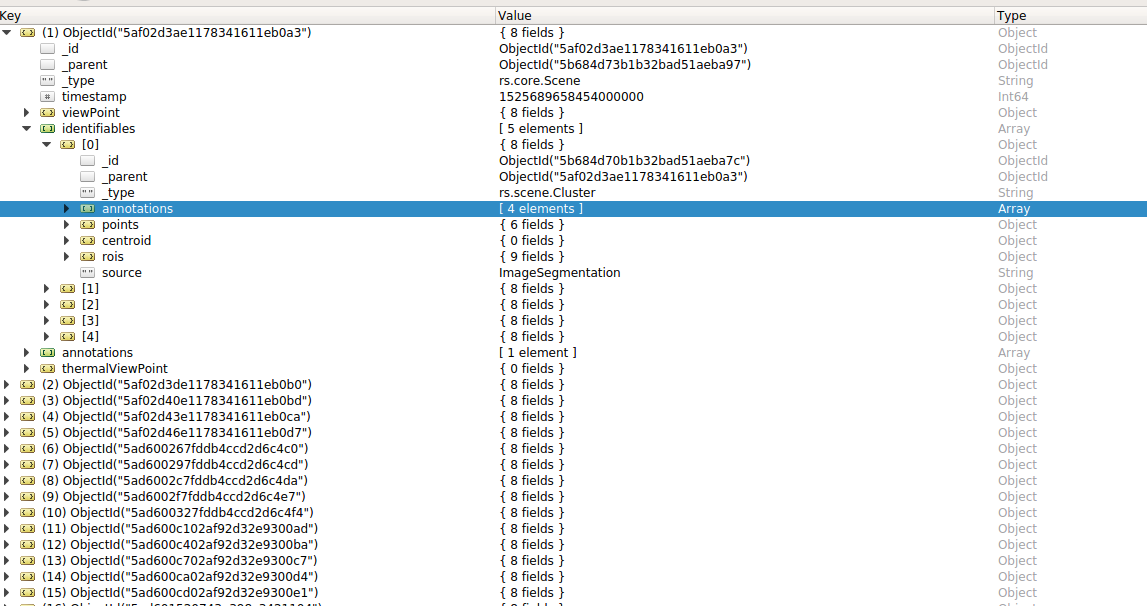
\includegraphics[width=\textwidth]{img/chapter3/mongoPic.png}
\caption[Die scene Collection einer \mongodb-Instanz]{Beispielhafte scene Collection, die von \robosherlock in einer \mongodb-Instanz während dieser Arbeit angelegt wird. Das geöffnet Dokument enthält Informationen zu dem ersten bearbeiteten Bild. Unter \textit{identifiables} werden die einzelnen Objekthypothesen und Informationen zu ihnen abgespeichert. Das Highlight zeigt das Dokument für die Annotationen des Clusters.}
\end{figure}

\robosherlock ist in der Lage seine Daten in einer laufenden \mongodb-Instanz zu speichern. Kern ist dabei die \gls{cas} Collection. Diese beinhaltet Referenzen zu den anderen relevanten \textit{views}. Dies sind Daten eines Sensors, wie das \gls{rgb}-Bild oder die Objektmaske. Die \textit{scene} Collection enthält Informationen, was \robosherlock zu einem bestimmten Zeitpunkt wahrgenommen hat, unter anderem mit Informationen über den Zeitpunkt, den Viewpoint des Roboters, Objekthypothesen und Annotationen \cite{episodicMemory}.  



\section{Markov-Logik-Netzwerke}
\label{sec:mln}
\glspl{mln} kombinieren die Ausdrucksstärke der \gls{fo} mit der Effizienz von \glspl{pgm}, Unsicherheit und Inkonsistenz zu behandeln und haben deshalb in den letzten Jahren großen Anklang in der Wissenschaft gefunden. Gerade in nicht-deterministischen Umgebungen stoßen \gls{fo} und \gls{pgm} \glspl{kb} an ihre Grenzen: \gls{fo} mit seiner Datenbank ähnlichen Repräsentation ist unpraktisch und unzumutbar mit zufälligen Ereignissen umzugehen, während bei \glspl{pgm} die Anzahl an Zufallsvariablen fest, die Menge der Variablen zu Beginn jedoch meistens nicht bekannt ist. \cite{nyga17} \par 
Ein \gls{mln} besteht aus einer Menge von Formeln in \gls{fo} als \acrlong{kb} und einer reell-zahligen Gewichtung für jede Formel. Die möglichen Welten beschreiben alle möglichen Belegungen der Variablen innerhalb einer \gls{kb}. Eine Formel beschreibt eine \textit{Beschränkung (oder constraint)} auf eine Teilmenge der Welten. Normalerweise gelten Welten, die eine Formel verletzten, als unmöglich, sie tritt nicht auf. \glspl{mln} schwächen die constraints nun ab. Welten sind nicht unmöglich sondern weniger wahrscheinlich, wenn sie eine Formel verletzen. Die Gewichtung gibt an, wie stark ein constraint ist. Ein höheres Gewicht besagt, dass der Unterschied der Wahrscheinlichkeit zwischen einer Welt, die die Formel erfüllt, und einer Welt, die sie nicht erfüllt, größer ist; wie wichtig die Formel also ist \cite{mln}. Ein \gls{mln} kann nun ein \textit{\gls{mn}} aufspannen, indem für jedes Atom eine boolesche Variable eingeführt wird, die den Wahrheitswert des Atoms beschreibt. Dieses \gls{mn} repräsentiert eine Wahrscheinlichkeitsverteilung über alle möglichen Welten. Eine Welt kann als Vektor von booleschen Variablen gesehen werden, der jedem Atom einen Wahrheitswert zuordnet. Die Menge aller Welten ist folglich die Menge aller möglichen Kombinationen von Wahrheitszuweisungen der Atome \cite{nyga17}. \par
Über ein \gls{mln} kann Inferenz oder \textit{Reasoning} stattfinden beziehungsweise geschlussfolgert werden. Dies geschieht normalerweise nicht mit exakter Inferenz, da für die Berechnung über alle möglichen Welten iteriert werden muss, was in Anwendungsfällen schnell sehr viele werden können. Stattdessen werden approximierenden Verfahren wie \textit{MCMC} oder \textit{MC-SAT} verwendet. \cite{nyga17} \par  
Im Rahmen dieser Arbeit soll \robosherlock mit einem \gls{mln} über die Objekthypothesen schlussfolgern, um welches Objekt es sich handelt. Nyga et al. (\cite{pr2looking}) führen aus, warum \glspl{mln} für die Repräsentation von Wissen und Reasoning in einem Perzeptionsframework von Vorteil sind: 
\begin{itemize}
	\item \glspl{mln} sind in der Lage die Beziehung zwischen Objekten abzubilden, da sie gleichzeitig eine beliebige aber endliche Menge von Objekten berücksichtigen können.
	\item \glspl{mln} bilden sich ihrer Entscheidung durch die unabhängige Anwendung der Experten und können so Inkonsistenzen kompensieren.
	\item \glspl{mln} können Antworten zu beliebige Anfragen über jeden Aspekt innerhalb des Models liefern. 
	\item indem neue oder zusätzliche Annotationen zu den Objekthypothesen hinzugefügt werden, können diese einfach in ein \gls{mln} integriert werden.    
\end{itemize}   
Für eine ausführlichere Vorstellung von \glspl{pgm}, \gls{fo}, \glspl{mln} und Markov Netzwerken verweise ich den Leser auf \cite{jain, nyga17, mln}. \par 

\textbf{Besispiel}\label{mlnexample} Es folgt ein Beispiel für ein simples \gls{mln} übernommen von dem Beispiel\footnote{\url{http://www.pracmln.org/mlntutorial.html}} das zu dem Programm \pracmln gegeben ist mit kleinen Abwandlungen basierend auf einem Besipiel aus \cite{nyga17}. Inhalt des Beispiels ist es, die Korrelation zwischen Rauchen und Krebs zu modellieren und den Einfluss auf das soziale Umfeld. \par
Zuerst werden die Prädikate definiert. Sie definieren, dass eine Person raucht oder Krebs haben kann und zwei Personen Freunde sein können:
\begin{lstlisting}[backgroundcolor=\color{backcolour}]
Raucht(person)
Krebs(person)
Freunde(person,person)
\end{lstlisting}
Es folgen Regeln in \gls{fo}, die beschreiben, dass Krebs aus dem Rauchen folgt, eine Freundesbeziehung immer von beiden ausgeht und dass unter Freunden entweder beide oder keiner raucht. 
\begin{lstlisting}[backgroundcolor=\color{backcolour}]
Raucht(p) => Krebs(p)
Freunde(p1,p2) <=> Freunde(p2,p1)
Freunde(p1,p2) => (Raucht(p1) <=> Raucht(p2))
\end{lstlisting}
An diese Regeln können nun die Gewichtungen geschrieben werden, die die 'Korrektheit' der Formel beschreibt. Zum Beispiel haben Raucher typischerweise Krebs. Unter Freunden rauchen meistens beide oder keiner:
\begin{lstlisting}[backgroundcolor=\color{backcolour}]
1.2 Raucht(p) => Krebs(p)
0.7 Freunde(p1,p2) => (Raucht(p1) <=> Raucht(p2))
\end{lstlisting}  
Für eine beliebige Menge von Personen kann nun eine Anfrage zu einem beliebigen Aspekt innerhalb des Modells  gestellt werden. Zum Beispiel kann die Wahrscheinlichkeit dafür erfragt werden, dass Anna Krebs hat, unter der Bedingung, dass sie mit dem Raucher Bob befreundet ist, \lstinline[breaklines=true]{ P(Krebs(Anna)  | Freunde(Anna,Bob)  ^ Raucht(Bob))}, oder dass Celia mit Bob befreundet ist, unter der Bedingung, dass sie nicht raucht, \lstinline[breaklines=true]{P(Freunde(Celia,Bob)  | !Raucht(Celia))}.


\subsection{pracmln}
\label{subsec:pracmln}
Um ein \gls{mln} mit Trainingsdaten zu trainieren und darüber zu schlussfolgern, wird die Toolbox \pracmln\footnote{\url{http://www.pracmln.org/}} benutzt, das vom \gls{iai} der Universität Bremen entwickelt wird. \pracmln ist in Python geschrieben und bietet als ein Python Modul die Möglichkeit die Funktionen in eigenen Python-Skripten zu verwenden. \par 
Im folgenden wird das vorherige Beispiel (Seite \pageref{mlnexample}) ausgeweitet, indem es mit Trainingsdaten trainiert wird und Anfragen an das \gls{mln} gestellt werden. Das Beispiel hält sich dabei weiterhin an das Beispiel, das zu \pracmln gegeben ist.  \newline
In einem ersten Schritt müssen die Gewichtungen erlernt werden. Dazu werden Trainingsdaten benötigt. Im folgenden ist ein Auszug der im Beispiel verwendeten Trainingsdaten gegeben: 
\begin{lstlisting}[backgroundcolor=\color{backcolour}]
Friends(Anna, Bob)
Friends(Bob, Anna)
Friends(Anna, Edward)
Friends(Edward, Anna)  

Smokes(Anna)
Smokes(Edward)
Smokes(Frank)
Smokes(Gary)

Cancer(Anna)
Cancer(Edward)
\end{lstlisting}  
Im Learning-Tool von \pracmln kann zusammen mit dem vorher spezifizierten \gls{mln} und einer auswählbaren Lernmethode nun ein \gls{mln} antrainiert werden, das auch die Gewichtungen errechnet.     
\begin{lstlisting}[backgroundcolor=\color{backcolour}]
1.126769 Raucht(p) => Krebs(p)
1.577776 Freunde(p1,p2) => (Raucht(p1) <=> Raucht(p2))
\end{lstlisting}  
Es ist zu sehen, dass es mit den gegeben Daten typisch ist, das Raucher auch Krebs haben, noch typischer jedoch das unter Freunden geraucht oder nicht geraucht wird.\newline
Um nun Wissen aus der \gls{kb} zu inferieren, wird das Query-Tool benutzt. Hier wird eine Evidenz angegeben, also eine Bedingung für unsere Anfragen: Anna hat Krebs, Bob nicht und Freunde sind sie auch nicht. 
\begin{lstlisting}[backgroundcolor=\color{backcolour}]
Krebs(Anna)
!Krebs(Bob)
!Freunde(Anna,Bob)
\end{lstlisting} 
Nun können Anfragen gestellt werden, die das \gls{mln} unter Einbezug der Evidenz zu beantworten versucht. Dies Anfragen drehen sich um das Rauchverhalten von Anna und Bob: \lstinline[breaklines=true]{Raucht(Anna)}, \lstinline[breaklines=true]{Raucht(Bob)}, \lstinline[breaklines=true]{Raucht(Anna)  ^ Raucht(Bob)}, \lstinline[breaklines=true]{Raucht(Anna)  v Raucht(Bob)}. \newline
Es kann mit exakter Inferenz folgendes berechnet werden: 
\begin{lstlisting}[backgroundcolor=\color{backcolour}]
0.436830  Raucht(Anna)
0.152667  Raucht(Anna) ^ Raucht(Bob)
0.528921  Raucht(Anna) v Raucht(Bob)
0.244758  Raucht(Bob)
\end{lstlisting} 
Es ist zu sehen, dass Anna mit größerer Wahrscheinlichkeit raucht als Bob. Die wahrscheinlich das mindestens einer der Beiden raucht ist sogar noch höher. Jedoch ist es unwahrscheinlich das beide rauchen. \newline
Anstatt exakter Inferenz kann auch ein approximiertes Verfahren benutzt werden, was im Falle des Beispiels auch eine gute Annäherung bietet, bei einer kleinen Evidenz jedoch nicht nötig ist. Denn die Anzahl aller möglichen Welten beträgt lediglich $2^8 = 256$, was in im Gegensatz zu Anwendungsfällen noch gering ist. Das Query-Tool kann auch die möglichen Welten ausgeben. Im folgenden sind die ersten drei, also die wahrscheinlichsten Welten, abgebildet. Eine Welt in der Anna und Bob Rauchen, Krebs haben und Freunde sind ist mit $0,81\%$ am wahrscheinlichsten:
\begin{lstlisting}[backgroundcolor=\color{backcolour}]
1   0.81%   Freunde(Anna,Anna)  Freunde(Anna,Bob)  Freunde(Bob,Anna)  Freunde(Bob,Bob)
            Raucht(Anna)  Raucht(Bob)  Krebs(Ann)   Krebs(Bob)
            5.242963e+03 <- 8.56 <- 1.1 1.1 1.6 1.6 1.6 1.6
2   0.26%   Freunde(Anna,Anna)  Freunde(Anna,Bob)  Freunde(Bob,Anna)  Freunde(Bob,Bob)
            Raucht(Anna)  Raucht(Bob)  Krebs(Anna)   !Krebs(Bob)
            1.699132e+03 <- 7.44 <- 1.1 1.6 1.6 1.6 1.6
3   0.26%   Freunde(Anna,Anna)  Freunde(Anna,Bob)  Freunde(Bob,Anna)  Freunde(Bob,Bob)
            Raucht(Anna)  Raucht(Bob) !Krebs(Anna)   Krebs(Bob)
            1.699132e+03 <- 7.44 <- 1.1 1.6 1.6 1.6 1.6
\end{lstlisting}  